
\section{基于点云的三维深度生成模型}
\label{section:gen3d}
在前面的章节中%第 \ref{cha:3d_deep_learning}、\ref{cha:gen} 章中,
我们先后介绍了点云三维深度学习和深度生成模型,并展示了这两个领域已有的丰硕的成果。
那么一个自然的问题是:
我们能否将深度生成模型在图像生成等任务上的良好表现%出的非凡成果
迁移到点云的生成任务上呢?
本节所介绍的工作 \inlinecite{latentpc} 正是在这个方向上的探索与尝试。 %这样的。在此方向上的尝试。%上做出了一定的尝试。

在介绍本节工作前,我们有必要对%本章以及第 \ref{cha:exp} 章的
记号的使用予以说明。
在前面的章节%第 \ref{cha:3d_deep_learning}、\ref{cha:gen} 章
中,我们曾用 $S = \{\bm p_i\}_{i=0}^{N - 1}
	= \{(x_i, y_i, z_i)^T\}_{i=0}^{N - 1}$ 表示点云数据,用
$\bm x$ 表示深度生成模型需要生成的数据。
而在本节和第 \ref{cha:exp}、\ref{cha:result} 章中,深度生成模型生成的数据恰好就是点云数据,因此我们将
视上下文算法的记号习惯,%灵活的
灵活地从 $\bm x$ 和 $S$ 中择一使用。但无论如何,这两者的本质是一样的。


\subsection{原始数据 GAN (Raw GAN, r-GAN) \label{section:rgan}}
一个直观的想法是:GAN 作为一个生成模型,其对于生成数据的形式没有任何假设。因此,我们可以
直接使用 %第 \ref{section:gan} 节中介绍的 
% GAN 来解决点云生成问题。%来完成点云生成的任务。
它解决点云生成问题。

正如我们在第 \ref{section:gan} 节介绍的, GAN 对于生成器网络 $G$ 和判别器网络 $D$ 的具体架构没有任何限定。
因此,为了使用 GAN,我们首先要因地制宜的设计好 $G$ 和 $D$ 的具体网络架构。
由于模型生成的对象是点云,因此我们可以参考第 \ref{cha:3d_deep_learning} 章中介绍的已有算法和网络架构。具体而言,
对于生成器网络 $S = G(\bm z; \bm \theta_G)$,第 $\ref{section:pointsetgen}$ 节中所介绍的 PointSetGen\cite{pointsetgen} 是一个不错的参考:我们可以借鉴 其 生成器部分,如全连接网络或者双分支网络。
而对于判别器网络 $D(S, \bm \theta_D)$,
我们可以直接使用第 $\ref{section:pointnet}$ 节中所介绍的 PointNet\cite{pointnet} 等架构。%能够出色的完成点云分类任务,因此。
固定了网络架构后,我们只要按照 GAN 的训练流程 \eqref{eq:ganloss0} 进行训练,就可以完成点云的生成任务。
我们将上述方法称为原始数据 GAN (Raw GAN, r-GAN)。

虽然 r-GAN 的流程直截了当,但它的实践效果并不好,如图 \ref{latent3drgan} 所示。
\begin{figure}[h]
	\centering%
	\subcaptionbox{真实数据\label{latent3dgt}}
	{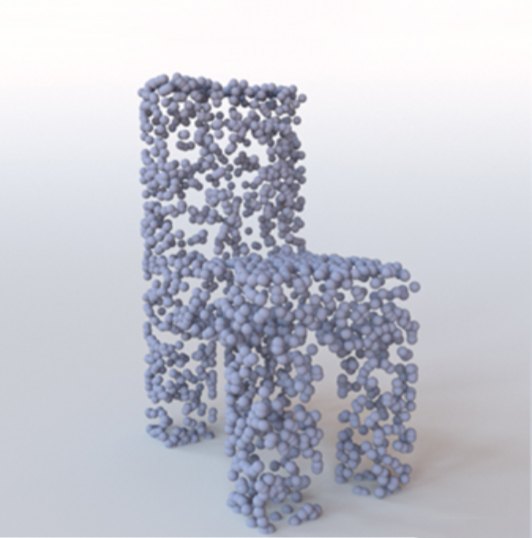
\includegraphics[width=.30\textwidth]{latent3dgt}}%
	\hspace{.5em}%
	\subcaptionbox{r-GAN\label{latent3drgan}}
	{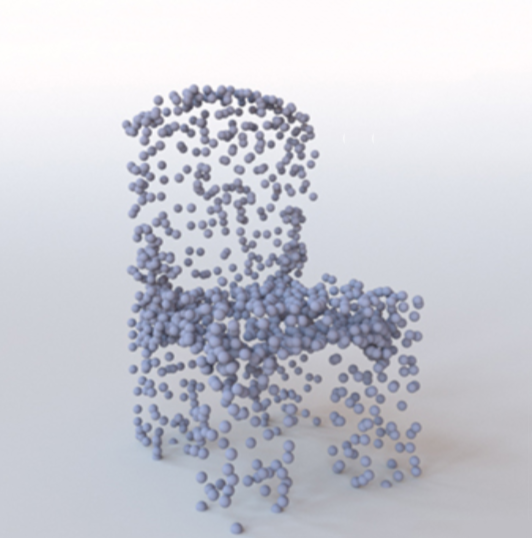
\includegraphics[width=.30\textwidth]{latent3drgan}}%
	\hspace{.5em}%
	\subcaptionbox{l-GAN\label{latent3dlgan}}
	{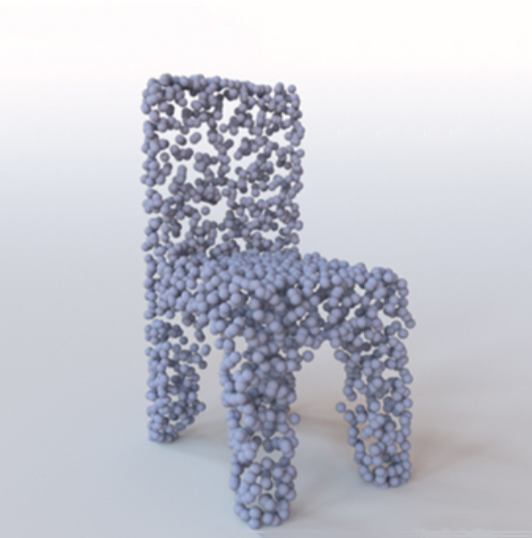
\includegraphics[width=.30\textwidth]{latent3dlgan}}%
	% \hspace{2em}%
	\caption{点云生成 \cite{latentpc}}
\end{figure}
在第 \ref{pointnet-robust} 节中,我们曾经介绍过 PointNet 的鲁棒性,即 PointNet 更关注点云数据的边、棱、角等关键信息,而忽略其他的非关键数据。
虽然这个性质有效提升了 PointNet 在点云分类、分割任务中的表现,但它对点云生成任务来说却是致命的。
%粗略地说,
粗略而言,在图 \ref{latent3drgan} 的例子中,椅子的棱角就是关键数据,而其内部点均为非关键数据。
由于 PointNet 会忽略掉非关键数据,因此作为判别器,它 %PointNet 
很难鉴定出椅面、椅背、椅子腿内部点的分布是否均匀合理,这也造成了图 \ref{latent3drgan} 中,点云集中在了某一区域如凳面上的问题。

\subsection{隐空间 GAN (Latent-space GAN, l-GAN)}
为了改善 r-GAN 的表现,我们可以先使用第 \ref{section:ae} 节中介绍的自编码器,提取点云的低维特征。

与 GAN 类似,自编码器同样是一种通用的模型,没有限制编码器 $E_{\text{AE}}$ 和解码器 $D_{\text{AE}}$ 的具体架构。
因此,我们%依然
同样可以取 $E_{\text{AE}}$ 为 PointNet,$D_{\text{AE}}$ 为 PointSetGen。而自编码器的损失函数 \eqref{eq:aeloss} 可以定义为点云的 Chamfer 距离 \eqref{eq:cd} 或推土机距离 \eqref{eq:emd}。
只要最小化此损失函数,我们就可以得到任意点云数据 $S = \bm x$ 的低维特征 $\bm z$。


然后,我们可以在点云的隐向量 $\bm z$ 上进行生成对抗训练,如图 \ref{fig:lgan} 所示。
\begin{figure}[h]
	\centering%
	{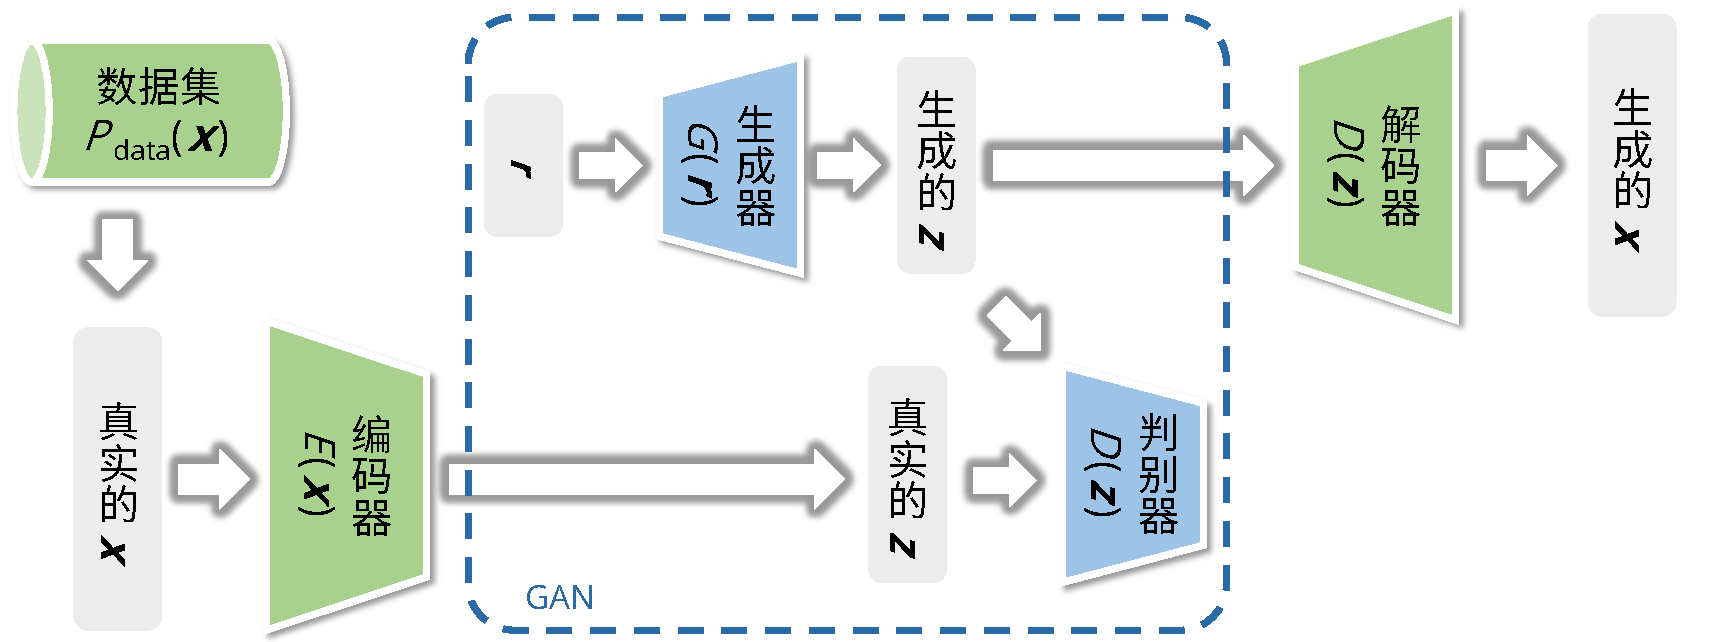
\includegraphics[width=.99\textwidth]{lgan}}%
	% \hspace{2em}%

	\caption{l-GAN 结构 \cite{latentpc}\label{fig:lgan}}
\end{figure}
我们认为:生成器从 $r \sim \NormDist(\bm 0, \bm I)$ 中生成隐向量 $\bm z = G_{\text{l-GAN}}(\bm r)$;
而判别器 $D_{\text{l-GAN}}(\bm z)$ 需要对于给定的隐向量 $\bm z$,判断它是从 $G_{\text{l-GAN}}$ 中生成的还是
从已有训练数据 $\bm x$ 提取的低维隐向量特征 $E_{\text{AE}}(\bm x)$。当需要从 $r \sim \NormDist(\bm 0, \bm I)$ 生成
实际的点云 $S = \bm x$时,我们需要经过生成器 $G_{\text{l-GAN}}$ 和解码器 $D_{\text{AE}}$ 两步映射:
\begin{align}
	S = \bm x = D_{\text{AE}}(\bm z) = D_{\text{AE}} \circ G_{\text{l-GAN}} (\bm r)
\end{align}
由于 GAN 生成的对象 $\bm z$ 已经是点云的低维特征了,因此我们而不必大费周章地再次使用 PointSetGen 和 PointNet 作为 $G_{\text{l-GAN}}$ 和 $D_{\text{l-GAN}}$ 的基本架构。事实上,仅使用简单的多层感知机,我们就%完全
可以达到较好的效果。
我们将上述方法称为隐空间 GAN (Latent-space GAN, l-GAN)。

l-GAN 在点云生成任务上的表现如 \ref{latent3dlgan} 所示,它解决了 PointNet 鲁棒性所带来的问题,质量较 r-GAN 相比有了一定的提升。


\subsection{Gauss 混合模型 (Gaussian Mixture Model, GMM)}
为了进一步提升生成点云的质量与覆盖率,工作 \inlinecite{latentpc} 还引入了隐向量 $\bm z$ 上的 Gauss 混合模型,作为 l-GAN 的改进版本。
但实验结果表明,与 l-GAN 相比,Gauss 混合模型的性能提升有限,其远远不如 r-GAN 到 l-GAN 的提升。%\cite{latentpc}。
限于篇幅原因,此处不再进一步展开介绍 Gauss 混合模型以及相关内容。%如何将其应用与三维点云生成的任务中。

% 与 r-GAN 相比,Gauss 混合模型的提升有限,同时不能很好地与 VAE/GAN 的工作结合,因此本文




% raw GAN

% l GAN
% 缺点,不能有效控制生成出的模型

